% Appendix Template

\chapter{Ejecución del algoritmo completa y detallada} % Main appendix title

\label{AppendixB} % Change X to a consecutive letter; for referencing this appendix elsewhere, use \ref{AppendixX}
En este apéndice, se detalla el procedimiento de ejecución de la última versión del algoritmo (sección \ref{sec:algoritmo4}) para un caso específico. 


\section{Ejecución del caso POPN}

Siguiendo los pasos mencionados en el apéndice \ref{AppendixA} se carga la red POPN previamente creada. 

\begin{figure}[H]
	\centering
	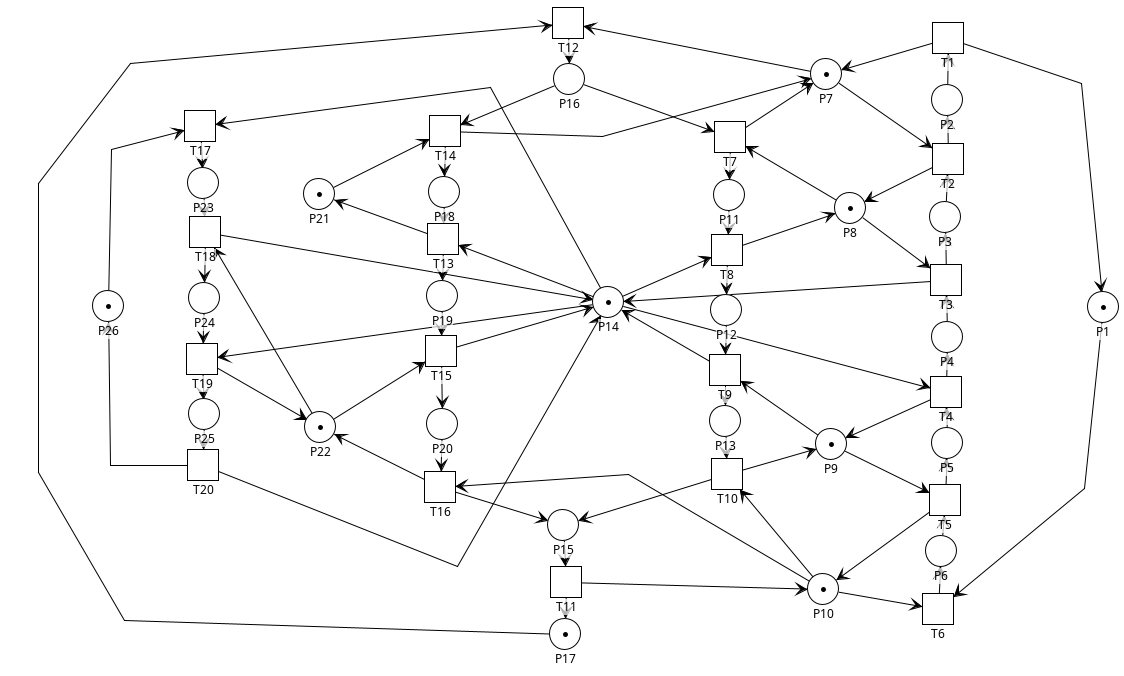
\includegraphics[scale=0.45]{Figures/apendiceB/POPN_DEADLOCK.png}
	\caption[RdP POPN]{RdP POPN \cite{libropopn}.}
	\label{fig:popndeadlocktrue}
 \end{figure}

En primera instancia se verifica la presencia de deadlock como se muestra en la figura \ref{fig:clasificacion-red}; al verificar que la red presenta deadlock \textbf{true} se prosigue con la extracción de los otros archivos necesarios:
\begin{itemize}
    \item Análisis de invariantes.
    \item Matrices.
    \item Grafo de alcanzabilidad.
    \item Sifones y trampas.
\end{itemize}

\noindent Se realiza la ejecución del algoritmo con \textit{Python v3}:
\begin{lstlisting}[language=SHELXL]
    		$ python3  algoritmo.py
\end{lstlisting}
\bigskip

\noindent Se solicita el ingreso de los archivos exportados del Petrinator (.html). Siendo:

\begin{itemize}
    \item go.html : Grafo de alcanzabilidad.
    \item mo.html : Matrices
    \item so.html : Sifones y trampas.
    \item io.html : Análisis de invariantes.
\end{itemize}
\bigskip

\noindent Al ser la primera vez que se ingresan los archivos se lleva a cabo la elección de la opción 1: \textit{Primer análisis de la red}. El cual solicita ingresar el nombre de la red con la extensión \textit{.pflow} a la que se le colocará el supervisor correspondiente.
Una vez procesada la información y llevado a cabo el análisis, el algoritmo arroja los siguientes resultados:
\bigskip

\begin{figure} [H]
    \centering
    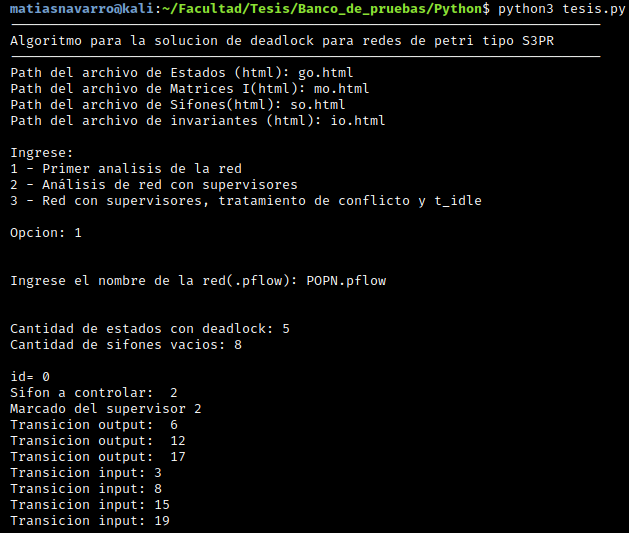
\includegraphics[scale=0.8]{Figures/apendiceB/Py-POPN1.png}
    \caption{Primer iteración: ejecución del primer análisis de la red.}
    \label{fig:b-popn1}
\end{figure}

\begin{figure} [H]
    \centering
    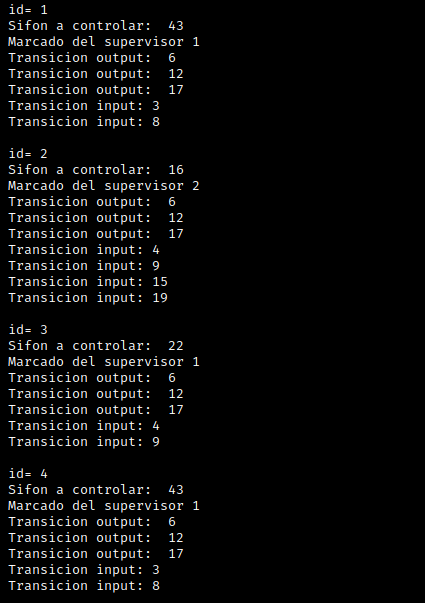
\includegraphics[scale=0.7]{Figures/apendiceB/Py-POPN2.png}
    \caption{Lista de supervisores.}
    \label{fig:b-popn2}
\end{figure}

\begin{figure} [H]
    \centering
    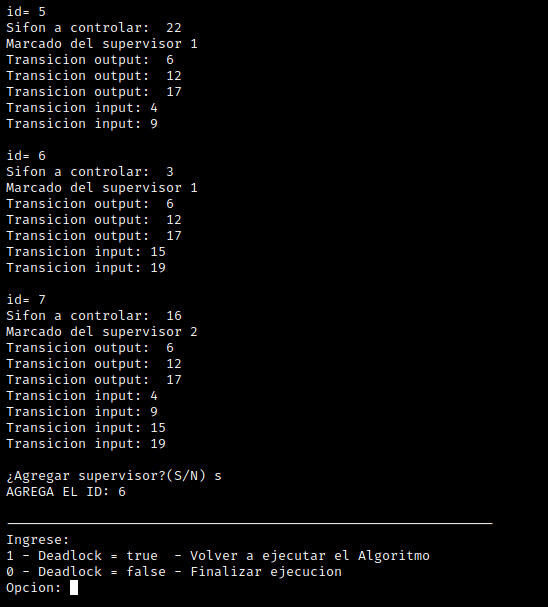
\includegraphics[scale=0.65]{Figures/apendiceB/Py-POPN3.png}
    \caption{Elección del supervisor.}
    \label{fig:b-popn3}
\end{figure}

El mismo arroja la cantidad de estados que presentan deadlock, el número de sifones vacíos asociados y los correspondientes supervisores para controlarlos cada uno con su respectivo id, marcado y transiciones input/output. \\
Una vez seleccionado el supervisor a colocar, el propio algoritmo se encarga de agregar la plaza con su marcado y arcos correspondientes al mismo sobre el archivo \textit{.pflow} especificado con anterioridad. \\
Luego se vuelve al Petrinator y se selecciona la opción \textit{Reload} como se muestra en la figura \ref{fig:b-reload}.

\begin{figure} [H]
    \centering
    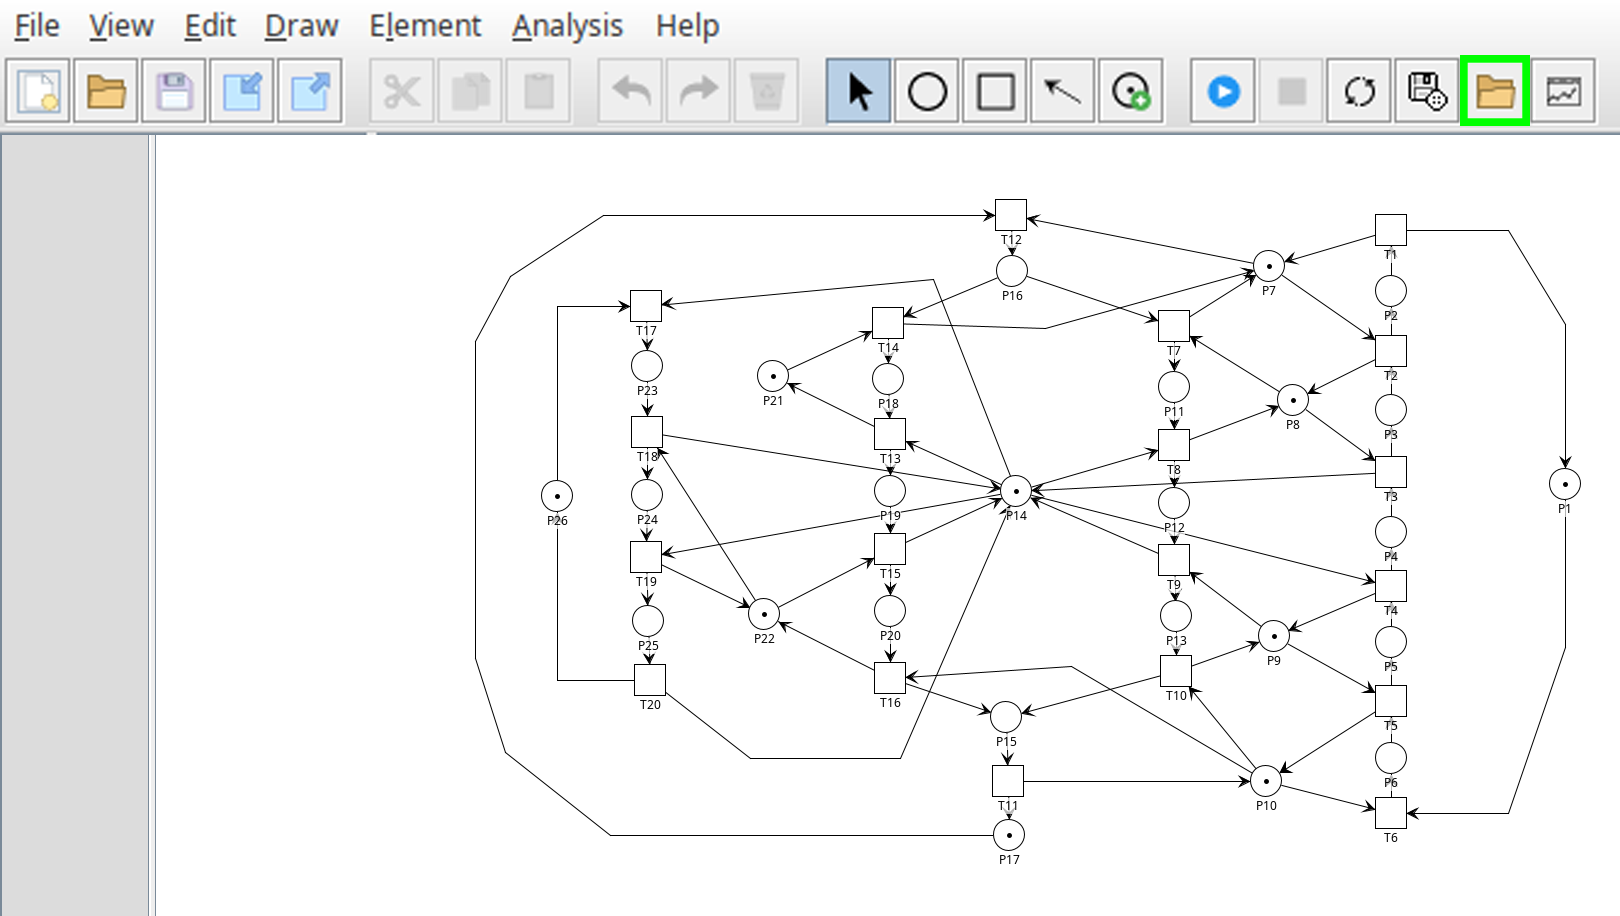
\includegraphics[width=\textwidth]{Figures/apendiceB/POPN_reload.png}
    \caption{Reload de la red.}
    \label{fig:b-reload}
\end{figure}

\noindent Como se muestra en la siguiente figura \ref{fig:b-supervisor}, la plaza resaltada $P_{27}$ es el supervisor agregado.

\begin{figure} [H]
    \centering
    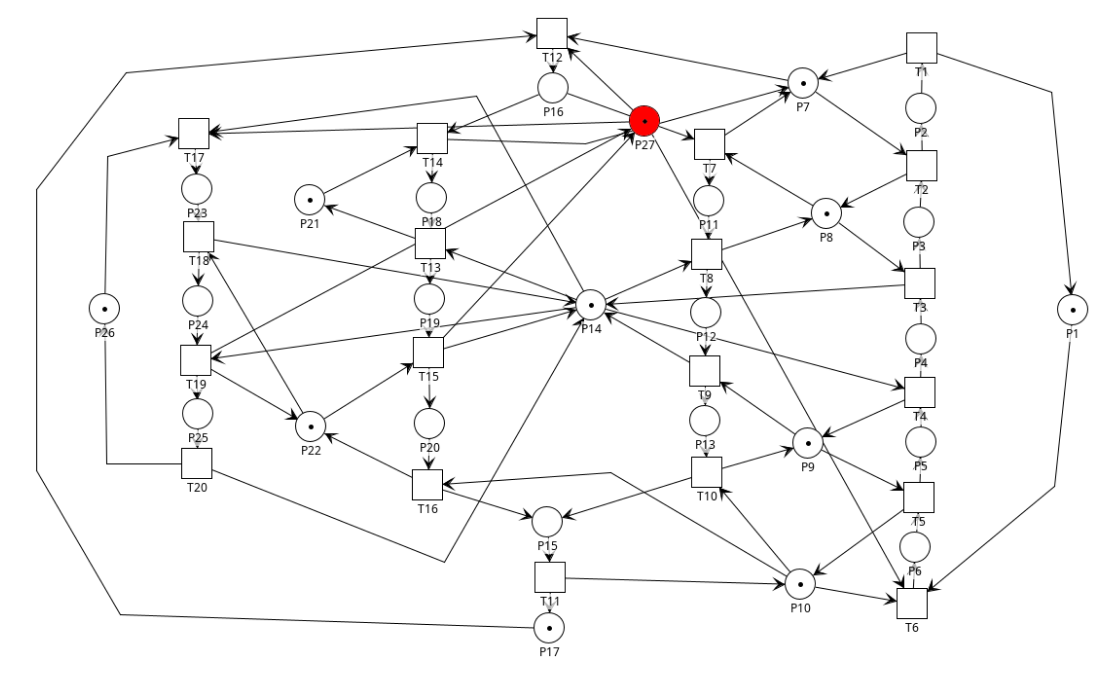
\includegraphics[scale=0.45]{Figures/apendiceB/Primer-supervisor.png}
    \caption{Supervisor agregado.}
    \label{fig:b-supervisor}
\end{figure}

Se debe verificar si el supervisor colocado soluciona el problema de deadlock realizando nuevamente el análisis de la red. En caso de no ser así, siguen existiendo el deadlock, se deberán extraer nuevamente los archivos correspondientes a la nueva red. Para seguir ejecutando el análisis se debe ingresar la opción 1 como se muestra al final de la figura \ref{fig:b-popn3}. \\
\par
Nuevamente, se deben ingresar los archivos para realizar un nuevo análisis. En este caso la segunda opción \textit{Análisis de red con supervisores}. 
\bigskip

\begin{figure} [H]
    \centering
    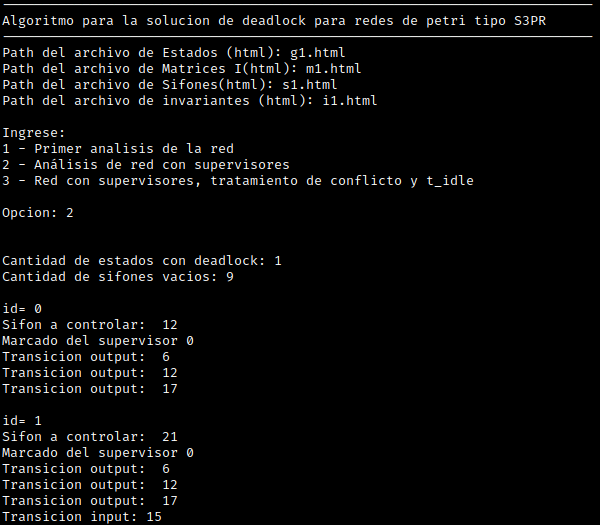
\includegraphics[width=\textwidth]{Figures/apendiceB/Py-POPN4.png}
    \caption{Segunda Iteración: análisis de la red con supervisores.}
    \label{fig:b-popn4}
\end{figure}
\bigskip

Como se puede observar en la figura \ref{fig:b-popn4} la lista de supervisores sugeridos presentan marcado 0, por este motivo no se coloca ninguno de estos y se vuelve a ejecutar el algoritmo pero haciendo uso de la opción \textit{Red con supervisores, tratamiento de conflicto y t\_idle}. Se deben eliminar/colocar los arcos indicados por el algoritmo como se muestra en la figura siguiente.

\begin{figure} [H]
    \centering
    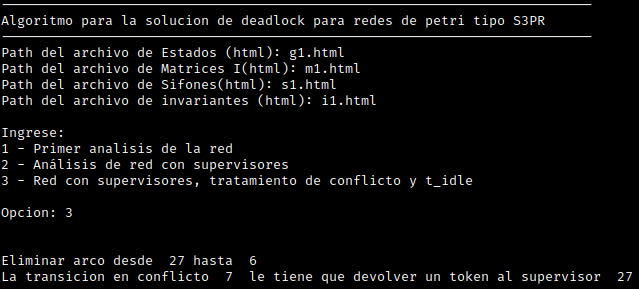
\includegraphics[width=\textwidth]{Figures/apendiceB/Py-POPN5.png}
    \caption{Tercera Iteración: red con supervisores, tratamiento de conflicto y t\_idle.}
    \label{fig:b-popn5}
\end{figure}

\noindent El resultado de lo indicado con anterioridad se observa en la siguiente imagen.

\begin{figure} [H]
    \centering
    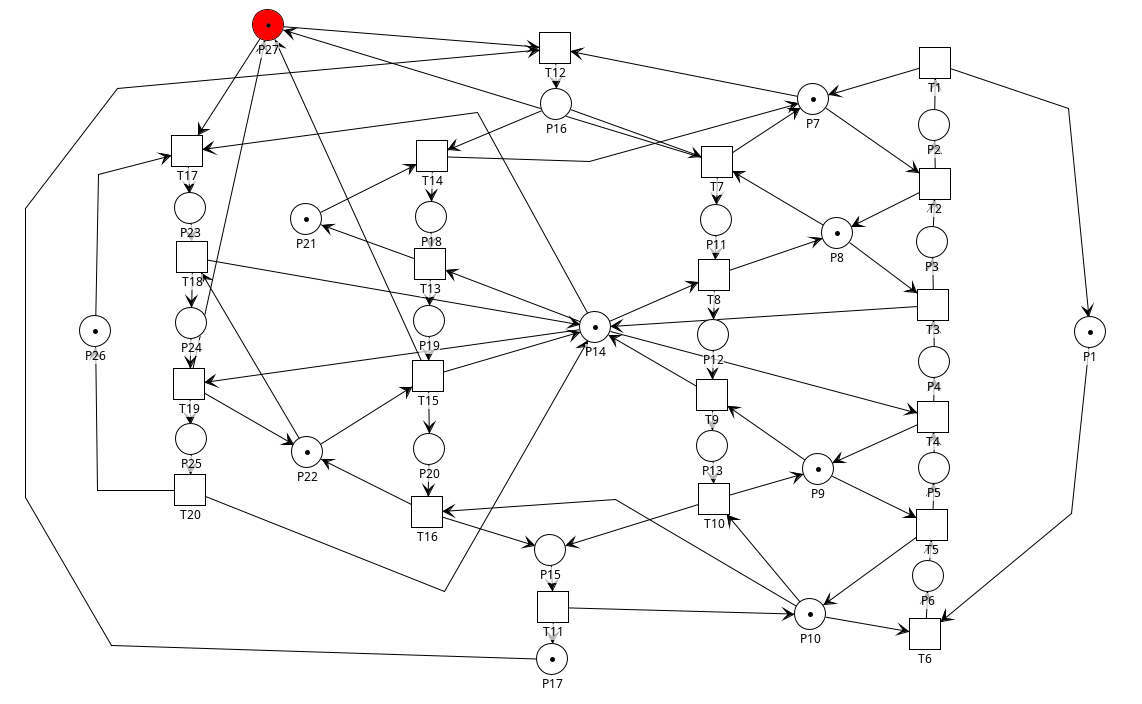
\includegraphics[width=\textwidth]{Figures/apendiceB/eliminacion-arco.png}
    \caption{Red resultante de agregar/eliminar arcos}
    \label{fig:b-supervisor1}
\end{figure}

Se verifica nuevamente si la red presenta deadlock y se extraen los archivos correspondientes. Para continuar con la ejecución iterativa hasta lograr el control total de la red, como se ejemplifica en las siguientes imágenes:  

\begin{figure} [H]
    \centering
    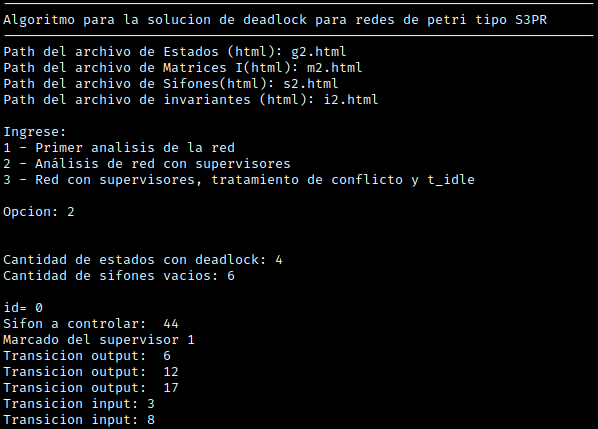
\includegraphics[width=\textwidth]{Figures/apendiceB/Py-POPN6.png}
    \caption{Cuarta iteración: análisis de la red con supervisores.}
    \label{fig:b-popn6}
\end{figure}

\begin{figure} [H]
    \centering
    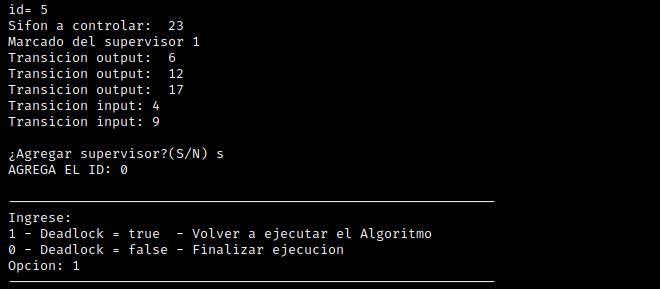
\includegraphics[width=\textwidth]{Figures/apendiceB/Py-POPN7.png}
    \caption{Elección del supervisor.}
    \label{fig:b-popn7}
\end{figure}

En este caso, se selecciona el supervisor de id = 0. Como se puede observar en la siguiente figura.

\begin{figure} [H]
    \centering
    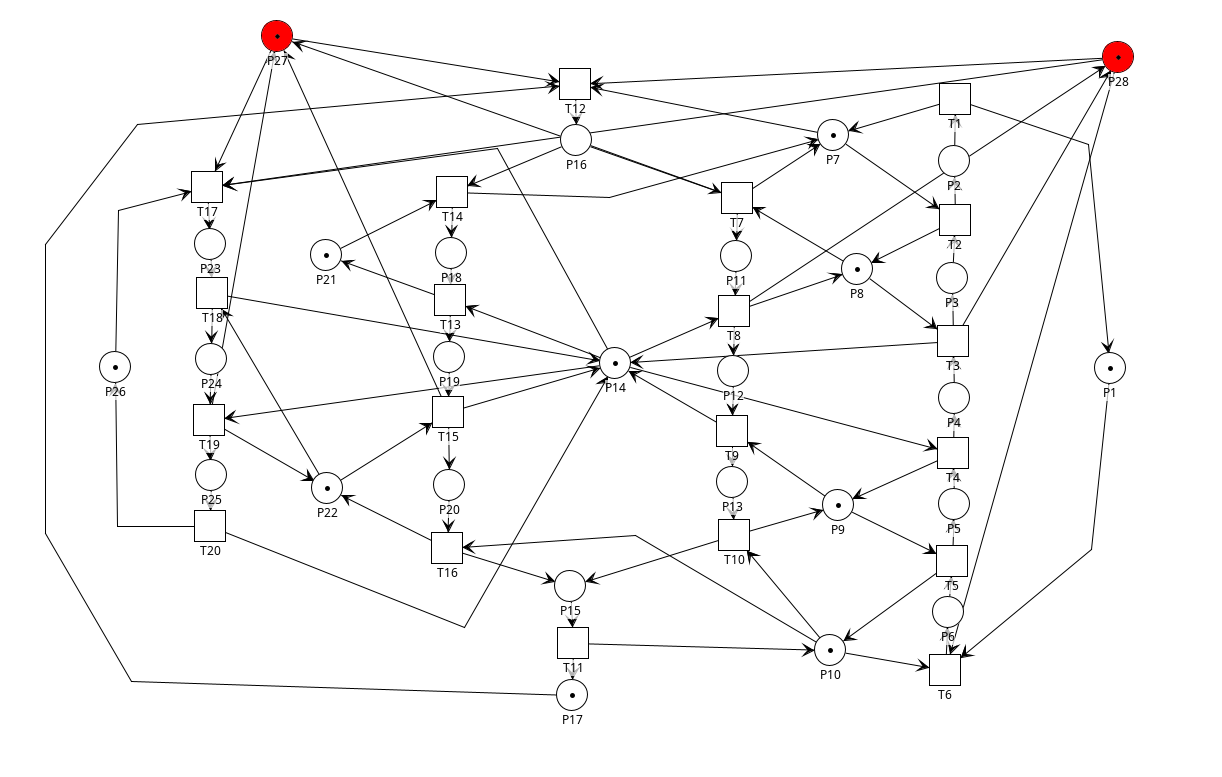
\includegraphics[width=\textwidth]{Figures/apendiceB/supervisor2.png}
    \caption{Segundo supervisor agregado.}
    \label{fig:b-supervisor2}
\end{figure}

De manera iterativa\footnote{Para cada nueva iteración fue necesario verificar si la red presentaba deadlock y exportar los archivos correspondientes, como en las iteraciones anteriores.} se colocan los demás supervisores, hasta que el análisis resulta con deadlock \textbf{false} o con supervisores de marcado 0. En el segundo caso, se debe hacer la ejecución de red con supervisores,tratamiento de conflicto y t\_idle.

\begin{figure} [H]
    \centering
    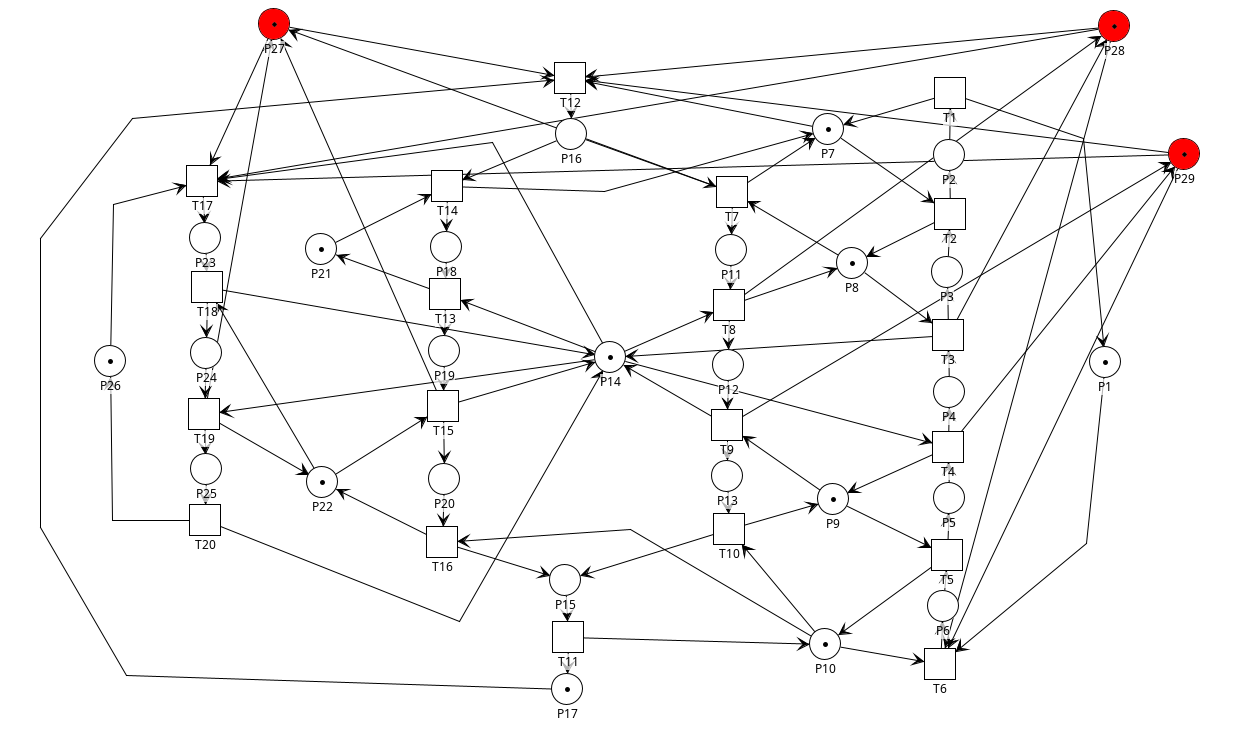
\includegraphics[width=\textwidth]{Figures/apendiceB/supervisor3.png}
    \caption{Tercer supervisor agregado.}
    \label{fig:b-supervisor3}
\end{figure}
\bigskip

\begin{figure} [H]
    \centering
    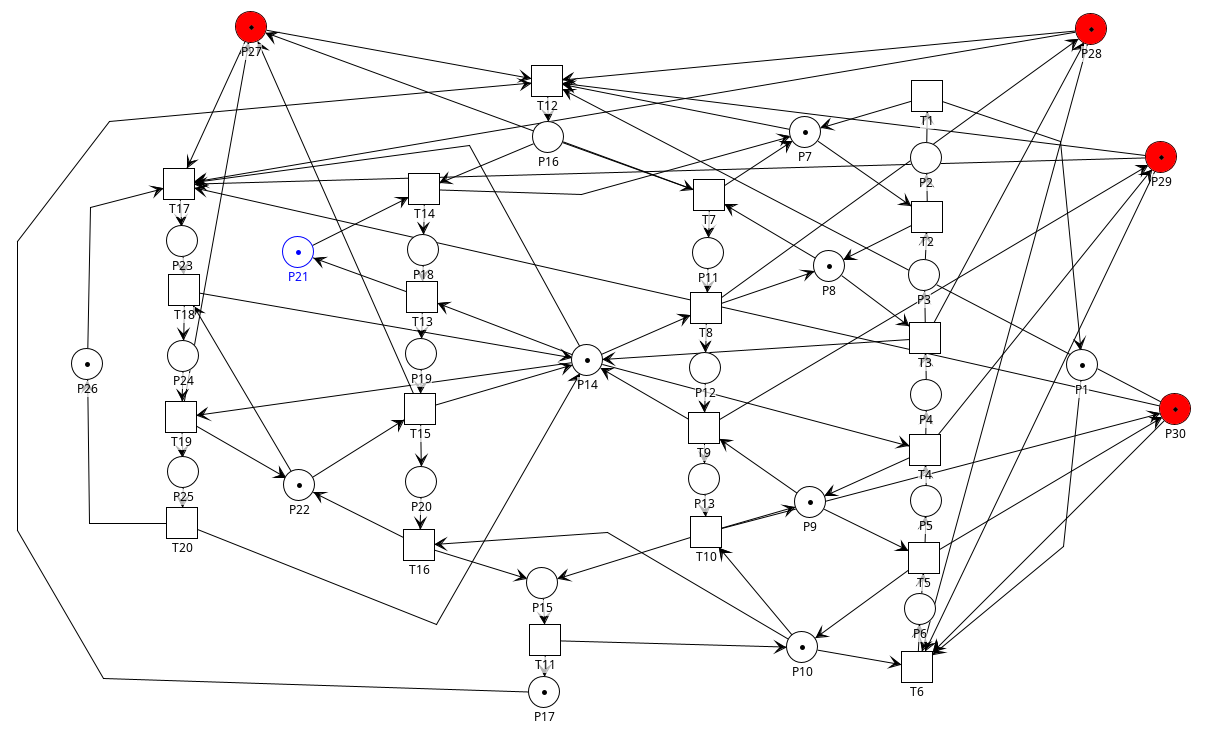
\includegraphics[width=\textwidth]{Figures/apendiceB/supervisor4.png}
    \caption{Cuarto supervisor agregado.}
    \label{fig:b-supervisor4}
\end{figure}

\begin{figure} [H]
    \centering
    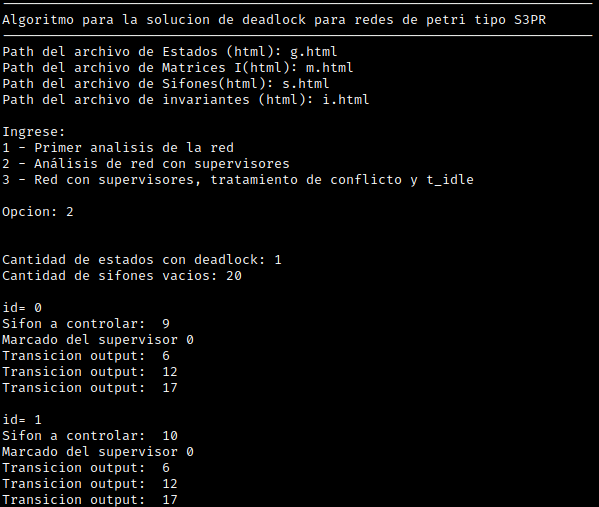
\includegraphics[width=\textwidth]{Figures/apendiceB/Py-POPN8.png}
    \caption{Última Iteración.}
    \label{fig:b-popn8}
\end{figure}

Por último, se ejecuta el algoritmo con la opción 3 como se observa en la figura \ref{fig:b-popn9}, indicando cuales arcos deben agregarse y cuales deben eliminarse. 

\begin{figure} [H]
    \centering
    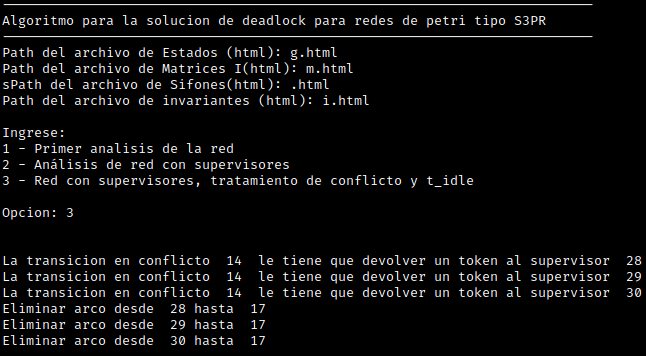
\includegraphics[width=\textwidth]{Figures/apendiceB/Py-POPN9.png}
    \caption{Arcos a eliminar/agregar.}
    \label{fig:b-popn9}
\end{figure}

Se agregan/eliminan los arcos y se comprueba la clasificación de la red observando que el deadlock es false. 

\begin{figure}[H]
	\centering
	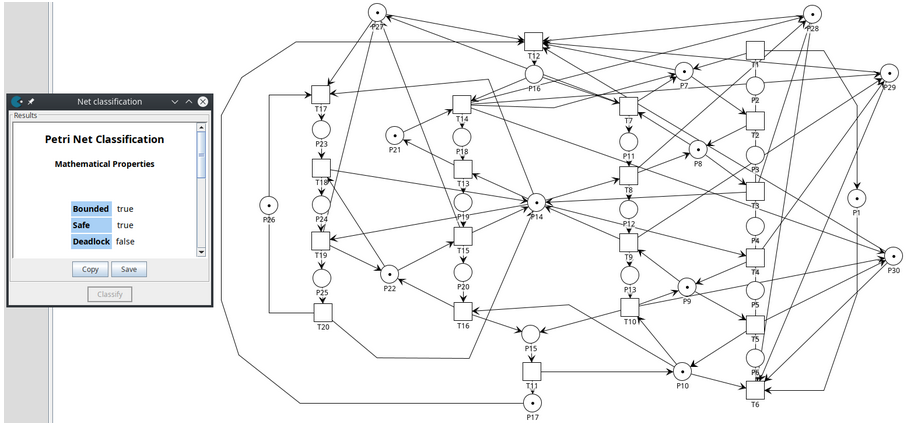
\includegraphics[width=\textwidth]{Figures/algoritmo4/popn_imag3.png}
	\caption{RdP POPN controlada.}
	\label{fig:Rdp-POPN-Contv4}
\end{figure}
\bigskip

Una vez que se verifica que la red no presenta deadlock, para finalizar la ejecución del programa, se debe ingresar \textit{0} en el menú de opciones que se muestra al final de la figura \ref{fig:b-popn3}. 